\chapter{Снова о многопроцессорности}
\section{Предъявите ваше состояние}
\begin{wrapfigure}{r}{0.35\linewidth}
    
\includegraphics[width=1\linewidth]{turkey.png}
\end{wrapfigure}
Примеры, показанные в предыдущей главе, годились для использования в качестве демонстрационного материала, но с таким ограниченным инструментарием далеко не уйдёшь.
Нет, примеры плохими не назовёшь, но от процессов и акторов пользы мало, когда они представлены только функциями и сообщениями.
Для устранения этого недостатка нам необходимо уметь сохранять в процессе состояние.

Давайте, для начала, создадим функцию в новом модуле \href{http://learnyousomeerlang.com/static/erlang/kitchen.erl}{kitchen.erl}, которая позволит процессу выполнять функции холодильника.
Процессу разрешено совершать две операции: хранить еду в холодильнике и вынимать её оттуда.
Вынимать можно только ту еду, которая была заранее помещена в холодильник.
Пусть основой нашего процесса будет следующая функция:
\begin{lstlisting}[style=erlang]
-module(kitchen).
-compile(export_all).
 
 fridge1() ->
     receive
         {From, {store, _Food}} ->
         From ! {self(), ok},
         fridge1();
     {From, {take, _Food}} ->
         %% uh....
         From ! {self(), not_found},
         fridge1();
     terminate ->
         ok
     end.
\end{lstlisting}

Что\--то здесь не так.
Когда мы делаем запрос на хранение еды, процесс возвращает результат \emph{ok}, но фактически еда нигде не сохраняется.
Будет вызвана функция \emph{fridge1()}, и она начнёт исполняться с чистого листа, без сохранённого состояния.
Очевидно также, что когда мы просим процесс извлечь еду из холодильника, её просто неоткуда взять, и остаётся просто вернуть в качестве результата \emph{not\_found}.
Ясно, что для хранения и извлечения провизии нам необходимо добавить в функцию состояние.

Благодаря рекурсии, состояние процесса может целиком содержаться в параметрах, которые передаются в функцию.
Для нашего процесса\--холодильника можно хранить весь провиант в виде списка, и когда кто\--нибудь захочет поесть, мы сможем поискать в нём необходимый продукт:
\begin{lstlisting}[style=erlang]
fridge2(FoodList) ->
    receive
        {From, {store, Food}} ->
            From ! {self(), ok},
            fridge2([Food|FoodList]);
        {From, {take, Food}} ->
            case lists:member(Food, FoodList) of
                true ->
                    From ! {self(), {ok, Food}},
                    fridge2(lists:delete(Food, FoodList));
                false ->
                    From ! {self(), not_found},
                    fridge2(FoodList)
            end;
        terminate ->
            ok
    end.
\end{lstlisting}

Сразу можно заметить, что \ops{fridge2/1} принимает один аргумент \--- \emph{FoodList}.
Когда мы пошлём сообщение вида \ops{\{From, \{store, Food\}\}} \--- функция добавит значение \emph{Food} в \emph{FoodList} перед следующей итерацией.
На следующей итерации рекурсивного вызова можно будет извлечь из списка тот же самый элемент, который мы туда поместили ранее.
Я даже реализовал эту возможность.
Функция использует \ops{lists:member/2} для проверки наличия \ops{Food} в \ops{FoodList}.
В зависимости от результата, полученный элемент либо пересылается вызывающему процессу (и удаляется из \emph{FoodList}), либо получателю отсылается атом \emph{not\_found}:
\begin{lstlisting}[style=erlang]
1> c(kitchen).
{ok,kitchen}
2> Pid = spawn(kitchen, fridge2, [[baking_soda]]).
<0.51.0>
3> Pid ! {self(), {store, milk}}.
{<0.33.0>,{store,milk}}
4> flush().
Shell got {<0.51.0>,ok}
ok
\end{lstlisting}

Функция хранения продуктов в холодильнике вроде бы работает.
Теперь попробуем поместить туда различные продукты, а затем их извлечь.
\begin{lstlisting}[style=erlang]
5> Pid ! {self(), {store, bacon}}.
{<0.33.0>,{store,bacon}}
6> Pid ! {self(), {take, bacon}}.
{<0.33.0>,{take,bacon}}
7> Pid ! {self(), {take, turkey}}.
{<0.33.0>,{take,turkey}}
8> flush().
Shell got {<0.51.0>,ok}
Shell got {<0.51.0>,{ok,bacon}}
Shell got {<0.51.0>,not_found}
ok
\end{lstlisting}

В соответствии с нашими ожиданиями, мы можем достать из холодильника бекон, потому что мы его туда поместили первым по счёту (вместе с молоком и пищевой содой), но когда мы просим процесс\--холодильник достать немного мяса индейки, у него ничего не выходит.
Именно поэтому мы получаем последнее сообщение \ops{\{<0.51.0>,not\_found\}}.
\section{Мы любим послания, но держим их в секрете}
\label{we-love-messages-but-we-keep-them-secret}
В предыдущем примере немного раздражает то, что программист, который собирается воспользоваться холодильником, должен иметь представление о протоколе, который был изобретён специально для этого процесса.
Что ведёт к усложнению без видимой на то необходимости.
Этот недостаток можно устранить, абстрагируя сообщения при помощи функций, которые эти сообщения получают и отправляют:
\begin{lstlisting}[style=erlang]
store(Pid, Food) ->
    Pid ! {self(), {store, Food}},
    receive
        {Pid, Msg} -> Msg
    end.
 
take(Pid, Food) ->
    Pid ! {self(), {take, Food}},
    receive
        {Pid, Msg} -> Msg
    end.
\end{lstlisting}

В таком виде взаимодействие с процессом выглядит гораздо опрятнее:
\begin{lstlisting}[style=erlang]
9> c(kitchen).
{ok,kitchen}
10> f().
ok
11> Pid = spawn(kitchen, fridge2, [[baking_soda]]).
<0.73.0>
12> kitchen:store(Pid, water).
ok
13> kitchen:take(Pid, water).
{ok,water}
14> kitchen:take(Pid, juice).
not_found
\end{lstlisting}

Нам больше не нужно переживать о том, как в принципе работают сообщения, нужно ли нам посылать \ops{self()} или какой\--то конкретный атом из числа \ops{take} или \ops{store}.
Мы должны знать лишь pid и то, какую функцию нужно вызвать.
Это позволяет спрятать подальше от глаз всю грязную работу и облегчает создание процесса\--холодильника.

Осталось только спрятать саму необходимость порождения процесса.
Мы позаботились о сокрытии сообщений, но обязанности по созданию процесса мы возложили на программиста.
Я добавлю следующую функцию \ops{start/1}:
\begin{lstlisting}[style=erlang]
start(FoodList) ->
    spawn(?MODULE, fridge2, [FoodList]).
\end{lstlisting}

\begin{wrapfigure}{r}{0.5\linewidth}
    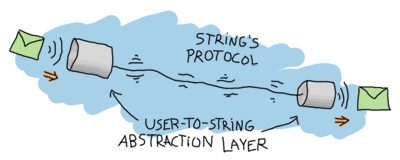
\includegraphics[width=1\linewidth]{abstraction.png}
\end{wrapfigure}
\ops{?MODULE} \--- это макрос, который возвращает имя текущего модуля.
Казалось бы, запись такой функции не несёт никаких преимуществ, но на самом деле некоторые преимущества есть.
Самым главным из них является согласованность с вызовами функций \ops{take/2} и \ops{store/2}.
Все операции процесса\--холодильника теперь обрабатываются модулем \href{http://learnyousomeerlang.com/static/erlang/kitchen.erl}{kitchen}.
Если вам необходимо добавить запись о времени старта процесса\--холодильника, или запустить второй процесс (к примеру, морозильник), то это можно легко сделать внутри нашей функции \ops{start/1}.
Но если порождение процесса будет делать пользователь при помощи \ops{spawn/3}, то в каждом месте, где запускается холодильник, мы будем обязаны добавить вызовы новых функций.
Здесь очень просто совершить ошибку, а ошибки это плохо.

Взглянем на эту функцию в деле:
\begin{lstlisting}[style=erlang]
15> f().
ok
16> c(kitchen).
{ok,kitchen}
17> Pid = kitchen:start([rhubarb, dog, hotdog]).
<0.84.0>
18> kitchen:take(Pid, dog).
{ok,dog}
19> kitchen:take(Pid, dog).
not_found
\end{lstlisting}

Ура!
Собака выбралась из холодильника, и наша абстракция готова к использованию!
\section{Тайм\--аут}
\label{time-out}
Давайте попробуем сделать кое\--что при помощи команды \ops{pid(A,B,C)}, которая позволяет нам преобразовать 3 целых числа \emph{A}, \emph{B} и \emph{C} в pid.
Попробуем намеренно передать функции \ops{kitchen:take/2} несуществующий pid:
\begin{lstlisting}[style=erlang]
20> kitchen:take(pid(0,250,0), dog).
\end{lstlisting}

Ой, оболочка зависла.
Зависание было вызвано реализацией функции \ops{take/2}.
Попробуем разобраться в произошедшем, и для начала рассмотрим события, которые происходят в случае нормального выполнения:
\begin{enumerate}
    \item От вас (от оболочки) пересылается сообщение процессу\--холодильнику, с указанием сохранить еду;
    \item Ваш процесс переключается в режим приёма и ожидает появления нового сообщения;
    \item Холодильник сохраняет элемент и посылает вашем процессу сообщение 'ok';
    \item Ваш процесс получает это подтверждение и продолжает заниматься своими делами.
\end{enumerate}
А вот что происходит при зависании оболочки:
\begin{enumerate}
    \item От вас (от оболочки) к неизвестному процессу уходит сообщение с указанием сохранить еду;
    \item Ваш процесс переключается в режим приёма и ожидает новое сообщение;
    \item Неизвестный процесс не существует вовсе, либо не ожидает получить ваше сообщение, и после его получения ничего с ним не делает;
    \item Процесс вашей оболочки застревает в режиме приёма.
\end{enumerate}
\begin{wrapfigure}{r}{0.15\linewidth}
    
\includegraphics[width=1\linewidth]{hourglass.png}
\end{wrapfigure}

Досадно, особенно если учесть, что эту ошибку нельзя обработать.
Ничего плохого не происходит, программа просто находится в режиме ожидания.
Как правило, любой код, имеющий дело с асинхронными операциями (а именно так организована передача сообщений в Erlang), должен иметь возможность прекращать ожидание по прошествии некоторого времени, если информация так и не была получена.
Похожую операцию проделывает веб\--браузер, когда загрузка страницы или изображения продолжается слишком долго.
Вы и сами проделываете то же самое, если при совершеннии телефонного звонка абонент долго не берёт трубку, или когда кто\--то не приходит на встречу вовремя.
Само собой, в Erlang на этот случай имеется соответствующий механизм, который является частью конструкции \ops{receive}.
\begin{lstlisting}[style=erlang]
receive
    Match -> Expression1
after Delay ->
    Expression2
end.
\end{lstlisting}

За выполнение того, о чём мы только что говорили, отвечает часть кода, которая находится между \ops{receive} и \ops{after}.
Код в \ops{after} будет выполнен, если за время равное \emph{Delay} (целое значение, заданное в миллисекундах) не будет получено сообщение, которое соответствует шаблону \emph{Match}.
В этом случае выполняется \emph{Expression2}.

Напишем пару новых функций интерфейса \ops{store2/2} и \ops{take2/2}, которые будут вести себя абсолютно так же как \ops{store/2} и \ops{take/2}, но прекращать ожидание после 3\--х секунд:
\begin{lstlisting}[style=erlang]
store2(Pid, Food) ->
    Pid ! {self(), {store, Food}},
    receive
        {Pid, Msg} -> Msg
    after 3000 ->
        timeout
    end.
 
take2(Pid, Food) ->
    Pid ! {self(), {take, Food}},
    receive
        {Pid, Msg} -> Msg
    after 3000 ->
        timeout
    end.
\end{lstlisting}

Теперь вы можете вывести оболочку из зависшего состояния нажатием Ctrl-G, и испытать новые интерфейсные функции:
\begin{lstlisting}[style=erlang]
User switch command
 --> k
 --> s
 --> c
Eshell V5.7.5  (abort with ^G)
1> c(kitchen).
{ok,kitchen}
2> kitchen:take2(pid(0,250,0), dog).
timeout
\end{lstlisting}

Вот теперь всё работает.\\
\colorbox{lgray}
{
\begin{minipage}{1.0\linewidth}
    \textbf{Замечание:} я говорил, что \ops{after} принимает значения только в миллисекундах, но ему также можно передавать атом \ops{infinity}.
    Во многих случаях от этой возможности мало проку (тогда выражение \ops{after} можно было бы полностью удалить), но иногда её используют, если программист имеет возможность передать время ожидания в функцию, в которой предполагается получение результата.
    Ожидание в такой ситуации действительно может продолжаться вечно, если этого захочет программист.
\end{minipage}
}

Кроме случаев, когда нужно прекращать слишком долгое ожидание, такие таймеры могут пригодиться и в других ситуациях.
Простым примером может послужить то, как работает функция \ops{\href{http://erldocs.com/R15B/timer.html\#sleep/1}{time:sleep/1}}, которую мы использовали ранее.
Вот как она реализована (поместим её в новый модуль \href{http://learnyousomeerlang.com/static/erlang/multiproc.erl}{multiproc.erl}):
\begin{lstlisting}[style=erlang]
sleep(T) ->
    receive
    after T -> ok
    end.
\end{lstlisting}

В \ops{receive} не будет найдено совпадение ни с одним из сообщений, так как для сопоставления с образцом не задан шаблон.
По истечении периода \emph{T} просто будет выполнена \ops{after} часть конструкции.

А вот ещё один особый случай, в котором время таймаута равно 0:
\begin{lstlisting}[style=erlang]
flush() ->
    receive
        _ -> flush()
    after 0 ->
        ok
    end.
\end{lstlisting}

В такой ситуации виртуальная машина Erlang будет пытаться найти сообщение, совпадающее с одним из указанных шаблонов.
В вышеприведённом случае может подойти что угодно.
Функция \ops{flush/0} будет рекурсивно вызывать себя до тех пор, пока в почтовом ящике не закончатся сообщения.
Когда ящик будет опустошён, выполнится код \ops{after 0 -> ok}, и функция завершит выполнение.
\section{Выборочный приём сообщений}
Рассмотренная  концепция 'смыва' (flushing) позволяет реализовать \emph{выборочный приём сообщений}, который даёт возможность назначать приоритет полученным сообщениям при помощи вложенных вызовов:
\begin{lstlisting}[style=erlang]
important() ->
    receive
        {Priority, Message} when Priority > 10 ->
            [Message | important()]
    after 0 ->
        normal()
    end.
 
normal() ->
    receive
        {_, Message} ->
            [Message | normal()]
    after 0 ->
        []
    end.
\end{lstlisting}

Эта функция построит список всех сообщений.
Первыми в нём будут стоять элементы с приоритетом больше 10:
\begin{lstlisting}[style=erlang]
1> c(multiproc).
{ok,multiproc}
2> self() ! {15, high}, self() ! {7, low}, self() ! {1, low}, self() ! {17, high}.      
{17,high}
3> multiproc:important().
[high,high,low,low]
\end{lstlisting}

Я использовал в коде условие \ops{after 0}, а значит процесс получит все сообщения до последнего.
Но он будет получать сообщения с приоритетом выше 10, совершенно не принимая в расчёт остальные послания.
А они будут накапливаться в \ops{normal/0}.

Если такой способ обработки вас заинтересовал, то имейте в виду. что иногда он может оказаться небезопасным из\--за особенностей работы выборочного приёма сообщений в Erlang.

Когда процессу отсылаются сообщения, они хранятся в почтовом ящике до тех пор, пока процесс не прочитает его и не сопоставит с шаблоном.
Как было сказано в \ref{the-hitchhikers-guide-to-concurrency} предыдущей главе, порядок хранения сообщений определяется  порядком их получения.
Так что когда вы попытаетесь провести над сообщением операцию сопоставления, это будет сообщение, полученное раньше всех остальных.
\begin{figure}[h!]
    \centering
    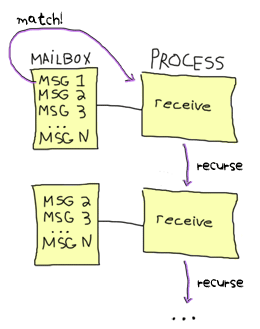
\includegraphics[width=0.35\textwidth]{msg-match.png}
\end{figure}

Самое старое сообщение сопоставляется с каждым шаблоном в \ops{receive}, пока совпадение не будет найдено.
После этого сообщение изымается из почтового ящика, и код процесса исполняется в обычном порядке до следующего \ops{receive}.
При обработке очередного \ops{receive}, виртуальная машина будет искать в почтовом ящике самое старое сообщение (следующее за тем, которое мы изъяли) и так далее.

Когда данное сообщение не совпадает ни с одним шаблоном, его помещают в \emph{очередь хранения} и переходят к следующему.
Если второе сообщение совпадает с одним из шаблонов, то первое снова помещается в вершину почтовой очереди, и будет обработано повторно чуть позже.
\begin{figure}[h!]
    \centering
    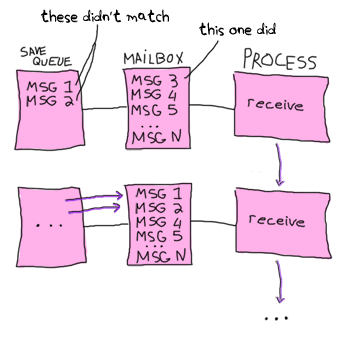
\includegraphics[width=0.5\textwidth]{msg-nomatch.png}
\end{figure}

Благодаря этому механизму, вы сможете сосредоточиться только на нужных вам сообщениях.
Способ игнорирования некоторых сообщений с целью последующей их обработки, описанный выше, как раз и является сущностью \emph{выборочного приёма сообщений}.
Не смотря на полезность этого метода, у него есть один недостаток: если процессу приходит много сообщений, которые никогда не понадобятся, то поиск нужных сообщений будет отнимать всё больше и больше времени (и размер процесса также будет увеличиваться).

Взгляните на рисунок, изображённый выше.
Представьте, что нам необходимо 367\--е сообщение, но предыдущие 366 \--- просто мусор, и наш код их проигнорировал.
Для получения 367\--го сообщения, процессу необходимо провести сопоставление для 366\--ти предшествующих сообщений.
Как только сопоставление проведено, и все ненужные сообщения были помещены в очередь, извлекается 367\--е сообщение, а все предыдущие 366 возвращаются обратно в почтовый ящик.
Следующее полезное сообщение может погрузиться ещё глубже и его придётся искать ещё дольше.

Эта проблема часто является причиной снижения производительности в Erlang.
Если ваше приложение исполняется медленно, и вы знаете, что оно пересылает много сообщений, то проблема может быть именно в этом.

Когда выборочный приём сообщений является причиной серьёзного замедления вашего кода, первым делом спросите себя, почему вы получаете сообщения, которые вам не нужны?
Посылаются ли эти сообщения нужным процессам?
Используете ли вы правильные шаблоны?
Может быть, сообщения отформатированы неверно?
Может, там, где необходимо использовать множество процессов, вы используете один?
Ответы на эти вопросы могут оказаться решением вашей проблемы.

Пытаясь уменьшить риск появления ненужных сообщений, загрязняющих почтовый ящик процесса, программисты на Erlang зачастую принимают меры, которые предотвращают появление таких событий.
Стандартный приём для такого случая выглядит следующим образом:
\begin{lstlisting}[style=erlang]
receive
    Pattern1 -> Expression1;
    Pattern2 -> Expression2;
    Pattern3 -> Expression3;
    ...
    PatternN -> ExpressionN;
    Unexpected ->
        io:format("unexpected message ~p~n", [Unexpected])
end.
\end{lstlisting}

Этот код заботится о том, чтобы любое сообщение совпало хотя бы с одним шаблоном.
Переменная \emph{Unexpected} будет захватывать любое неожиданное сообщение, изымать его из почтового ящика и отображать предупреждение об этом событии.
Скорее всего, вы захотите сохранить сообщение при помощи какого\--либо регистрирующего средства, чтобы впоследствии иметь возможность получить о нём информацию.
Было бы досадно навсегда потерять сообщения, отосланные по ошибке, а потом недоумевать, почему какой\--то из процессов не получил то, что должен был получить.

Если вам необходимо следить за приоритетом сообщений, и использование универсального шаблона не представляется возможным, то вы можете реализовать \href{http://en.wikipedia.org/wiki/Min-heap}{min\--кучу} или использовать модуль \ops{gb\_trees} для сохранения каждого полученного сообщения (проследите, чтобы приоритет стоял в ключе первым \--- так он будет задействован при сортировке).
Затем вы сможете просто извлекать \href{http://erldocs.com/R15B/gb_trees.html\#take_smallest/1}{наименьший} или \href{http://erldocs.com/R15B/gb_trees.html\#take_largest/1}{наибольший} элемент в структуре, в соответствии с вашими пожеланиями.

В большинстве случаев этот приём позволит извлекать сообщения с установленным приоритетом более эффективно, чем при помощи избирательного приёма сообщений.
Но если большинство получаемых сообщений имеют наибольший возможный приоритет, то этот метод может оказать на код замедляющее действие.
Как обычно, перед оптимизацией необходимо провести измерения и профилирование кода.\\
\colorbox{lgray}
{
\begin{minipage}{1.0\linewidth}
    \textbf{Замечание:} начиная с версии R14A, в компиляторе Erlang появилась новая оптимизация.
    Она упрощает избирательный приём сообщений для некоторых специальных случаев двустороннего взаимодействия процессов.
    Пример её использования можно найти в функции \ops{optimized/1} модуля \href{http://learnyousomeerlang.com/static/erlang/multiproc.erl}{multiproc.erl}.\\
    \\
    Чтобы эта оптимизация сработала, в функции необходимо создать ссылку (\ops{make\_ref()}) и отослать её в сообщении.
    Затем, в той же самой функции осуществляется избирательный приём сообщений.
    Так как ни одно сообщение не может совпасть с шаблоном, если оно не содержит сгенерированную ссылку, то компилятор автоматически заставляет виртуальную машину пропускать сообщения, полученные до момента создания этой ссылки.\\
    \\
    Заметьте, что вы не должны пытаться привести ваш код в соответствие с оптимизациями.
    Разработчики Erlang ищут часто используемые модели, и ускоряют их исполнение.
    Если вы пишете идиоматичный код, то оптимизации сами к вам придут.
    Не наоброт.
\end{minipage}
}

Теперь у нас есть представление о рассмотренных в этой главе концепциях, и на следующем этапе мы увидим как использовать обработку ошибок для нескольких процессов.
